\documentclass[a4paper,12pt]{article}
\usepackage[utf8]{inputenc} 
\usepackage[english,russian]{babel}
\usepackage{graphics}
\usepackage{epsfig}
\usepackage{amsmath,amssymb}


\usepackage[
  a4paper, mag=1000, nofoot,includehead, %, includefoot, nohead
  left=3cm, right=1.2cm, top=2cm, bottom=2.5cm, footskip=1cm, headsep=0.5cm
]{geometry}

\title{Measurement of \\B($J/\psi \to K^+K^-$)/B($J/\psi \to \mu^+\mu^-$) \\
with BES-3 detector}
\author{I.B. Nikolaev}


\newcommand{\ee}{e^{+}e^{-}}
\newcommand{\uu}{\mu^{+}\mu^{-}}
\newcommand{\KK}{K^{+}K^{-}}
\newcommand{\pipi}{\pi^{+}\pi^{-}}

\begin{document}
\maketitle

\section{Introduction}

\section{Event selection}

At first stage of selection no good neutral tracks and exactly four  charged which begin from interaction point tracks are selected:
\begin{itemize}
  \item $N_0 = 0$
	\item $N_q = 4$
	\item $|z| <  10$~cm,  $r_{xy} < 1$~cm. Here $z$ is the distance from poca track to interaction point along axis z, 
		and $r_{xy}$ is the distance from poca track to interaction point in the xy-plane.
	\item $|\cos{\theta}|<0.8$, where $\theta$ is the polar angle of charged track.
\end{itemize}


Two opposite charged tracks with momentum less 0.45~GeV is considered to be
$\pi^+$- and $\pi^-$- mesons candidates. This pion pair must have recoil
invariant mass in the window from 3.0 to 3.2 GeV.
\begin{itemize}
	\item $p<0.45$~GeV
	\item $3.0 < M_{rec} < 3.2$ GeV
\end{itemize}

\begin{figure}
\begin{center}
  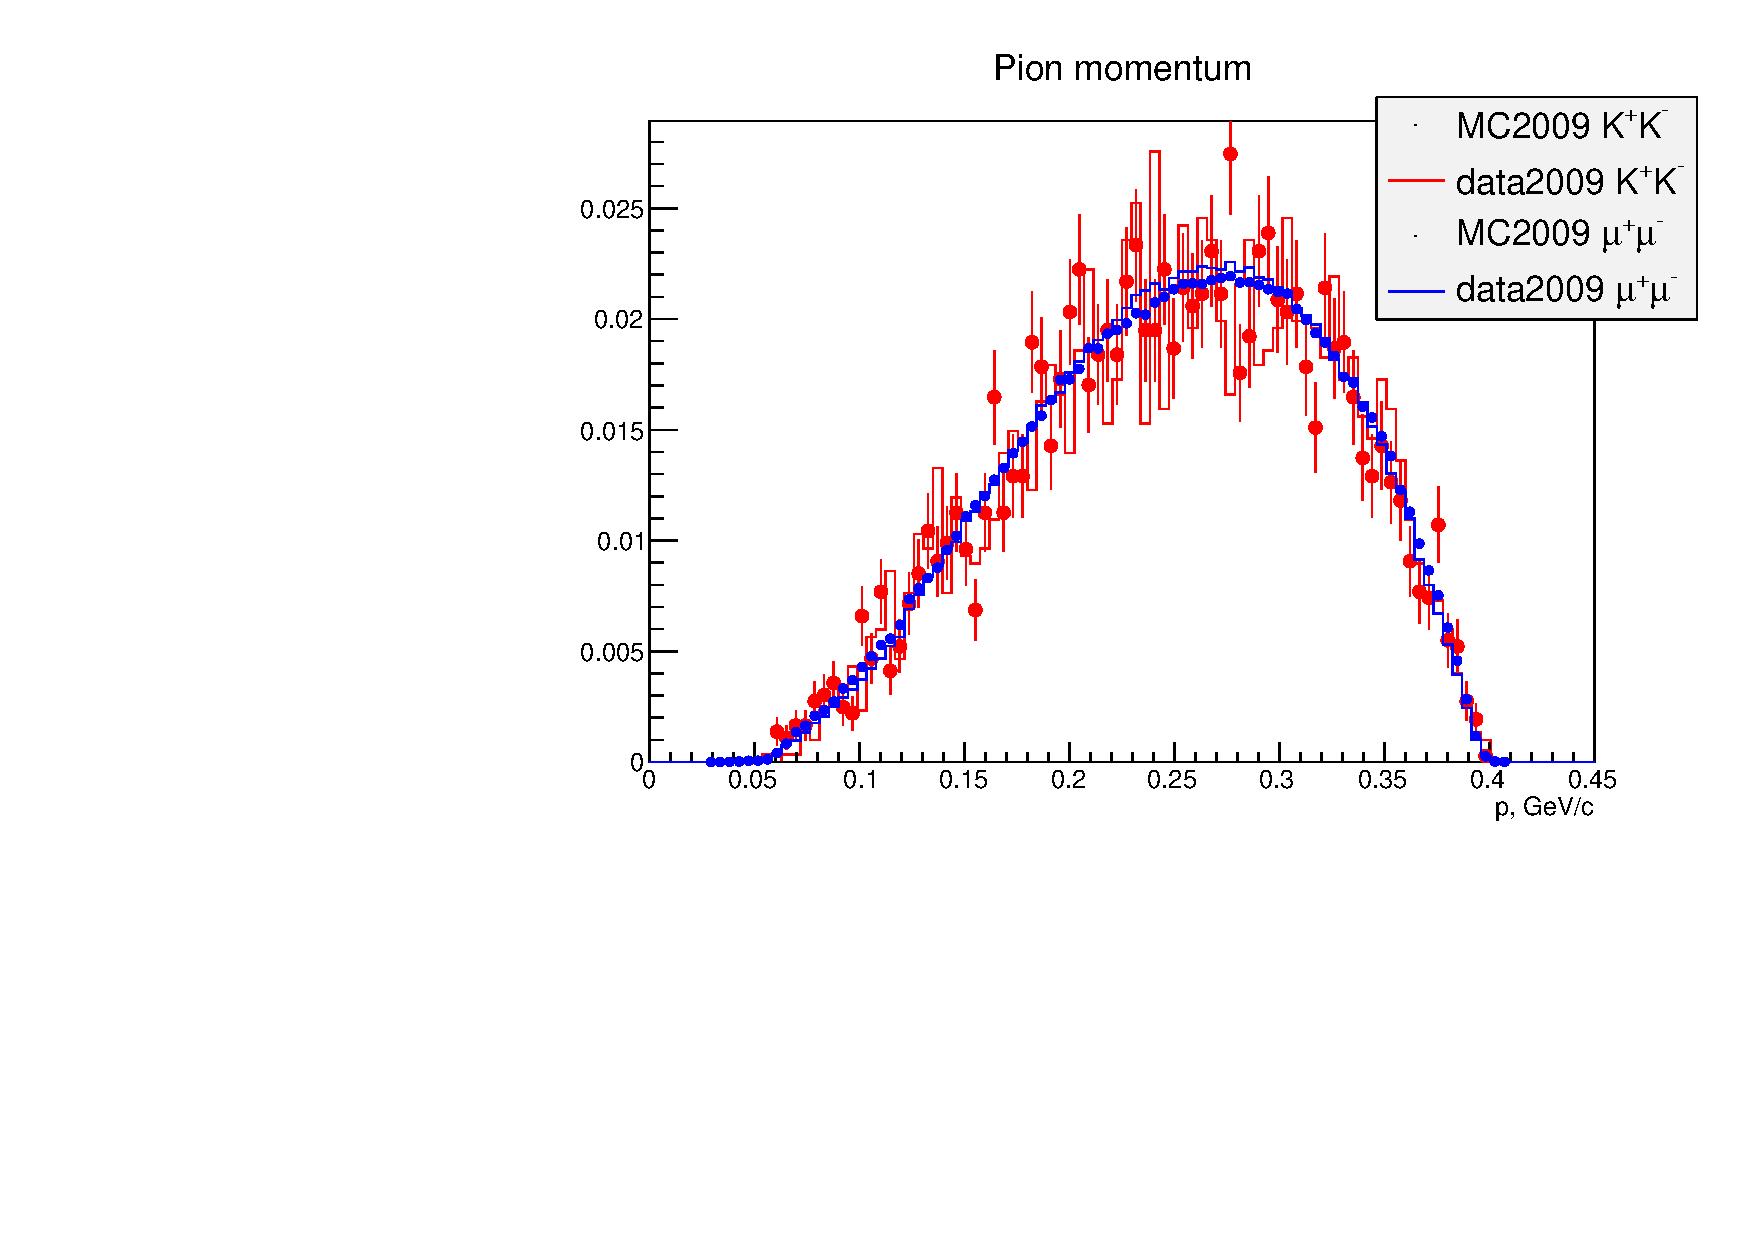
\includegraphics[width=0.48\textwidth]{fig/pion_momentum.pdf} \hfill
  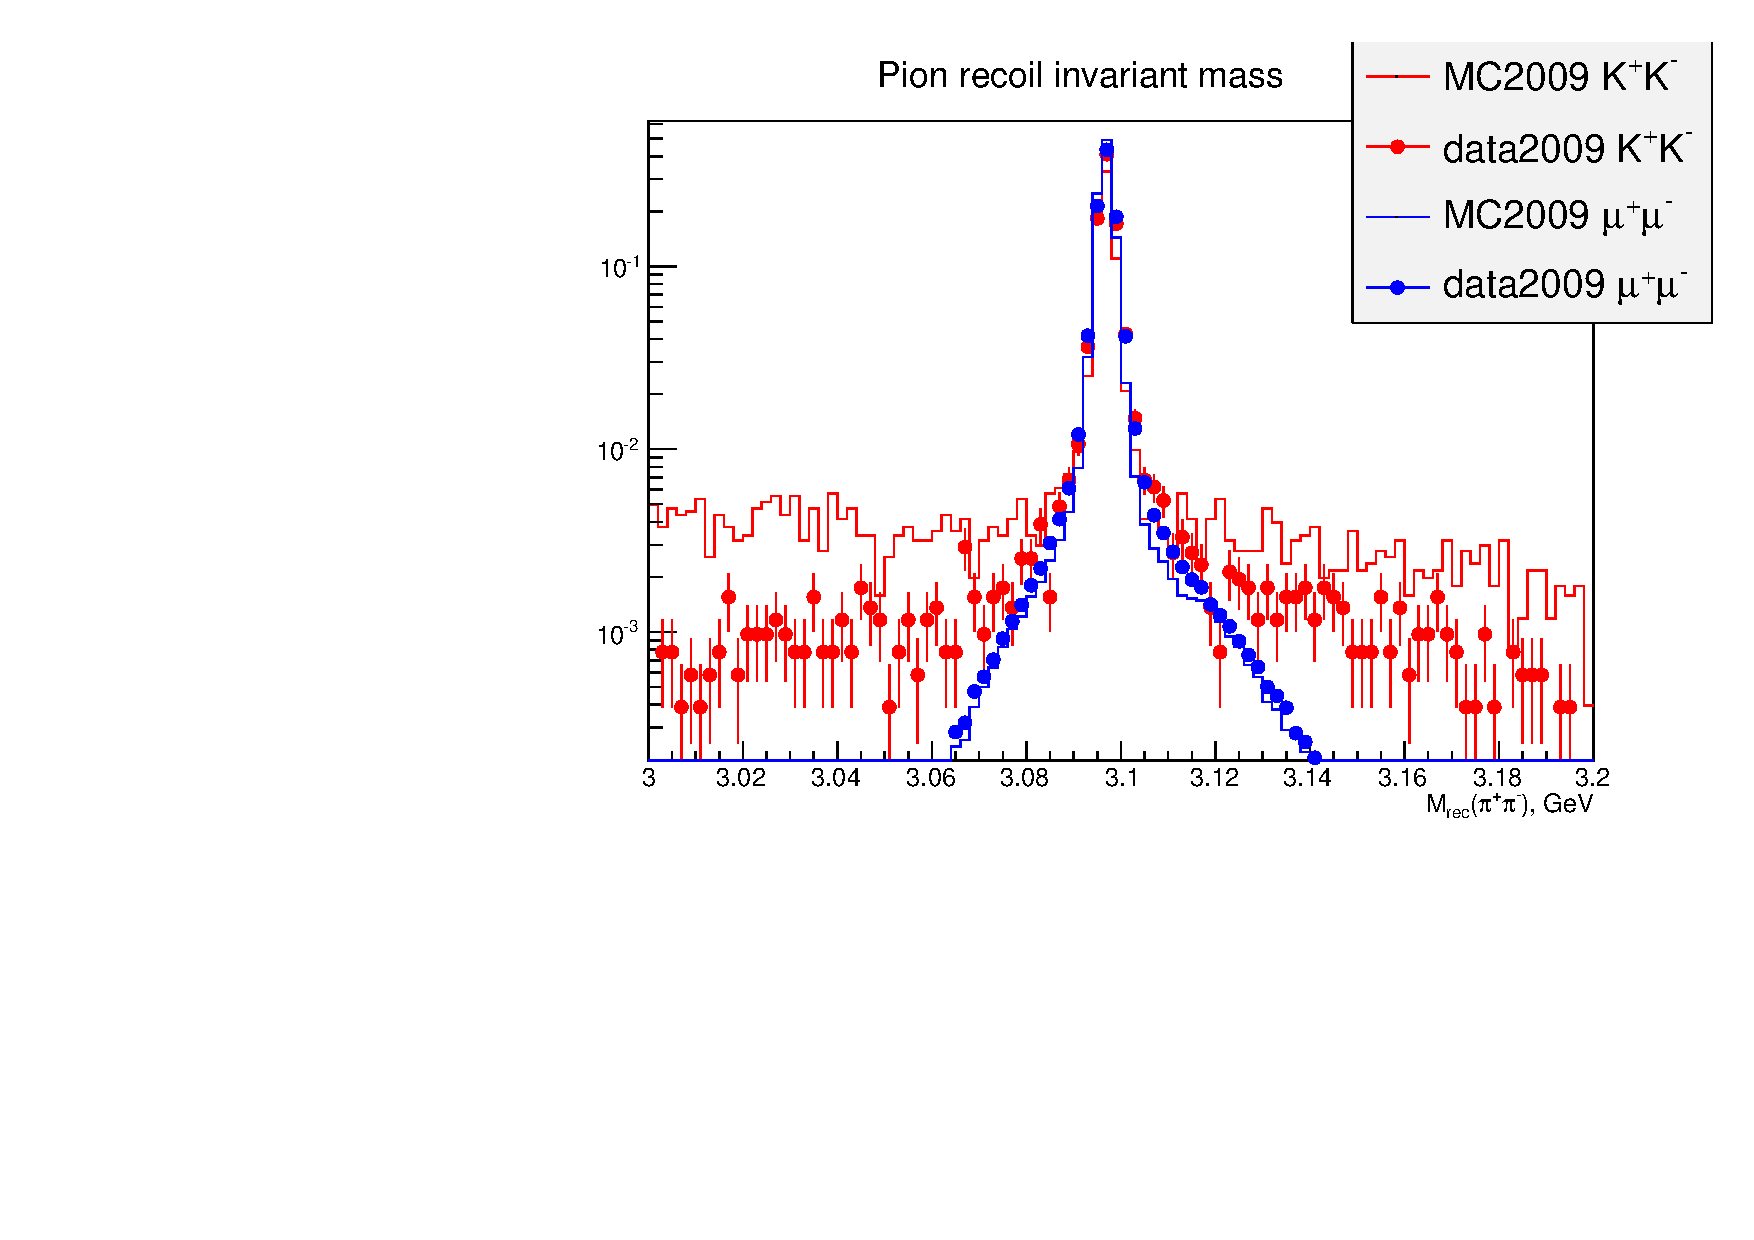
\includegraphics[width=0.48\textwidth]{fig/pion_Mrec.pdf}
  \caption{Pion momentum cut \mbox{$p<0.45$~GeV} is used. Pion recoil invariant mass cut $3.0 < M_{rec}(\pipi) < 3.2$~GeV is used}
\end{center}
\end{figure}

Two other particles must be opposite charged and have momentum more then 1.0
GeV and less 2 GeV. To suppress $\ee$ background E/p ratio must be less 0.8
GeV.
\begin{itemize}
	\item $1.0<p<2.0$~GeV
\end{itemize}

\begin{figure}
\begin{center}
  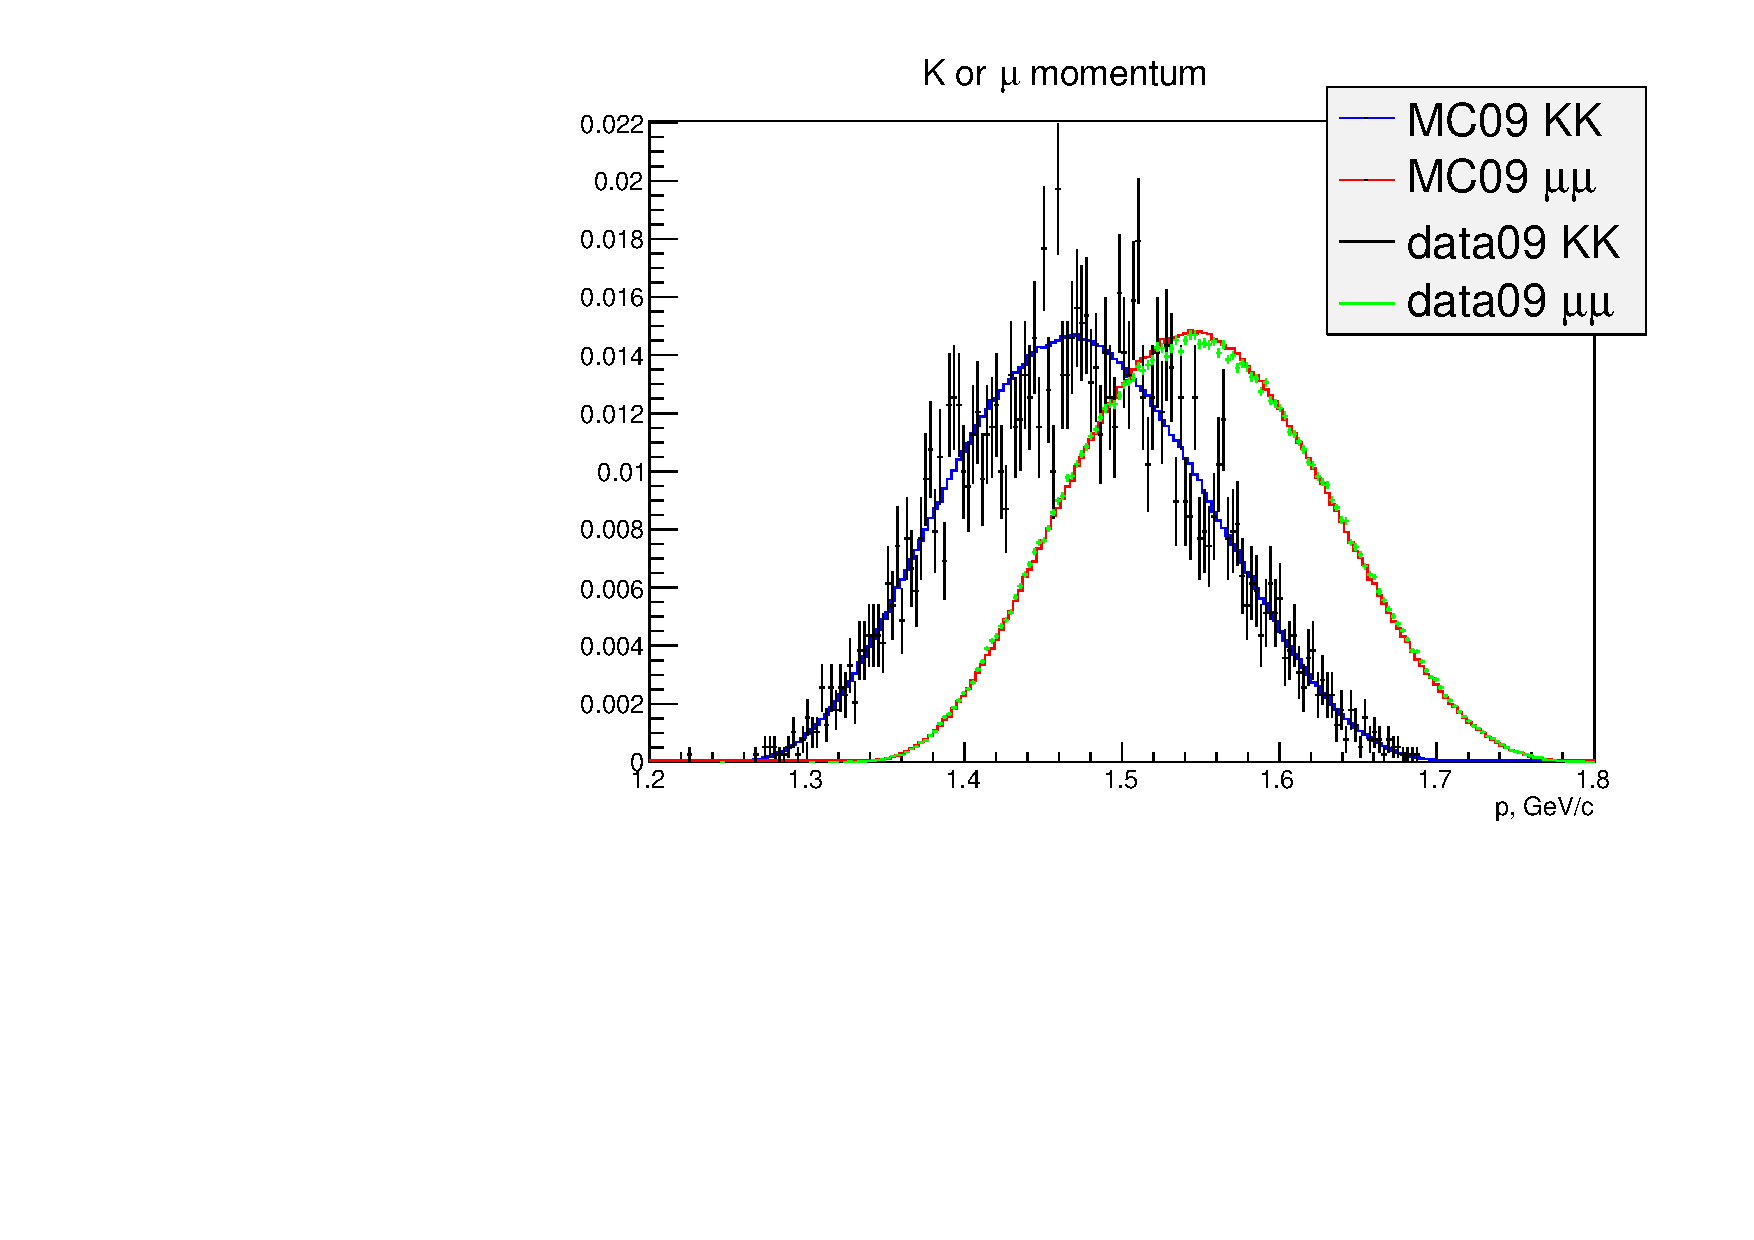
\includegraphics[width=0.48\textwidth]{fig/p.pdf} \hfill
  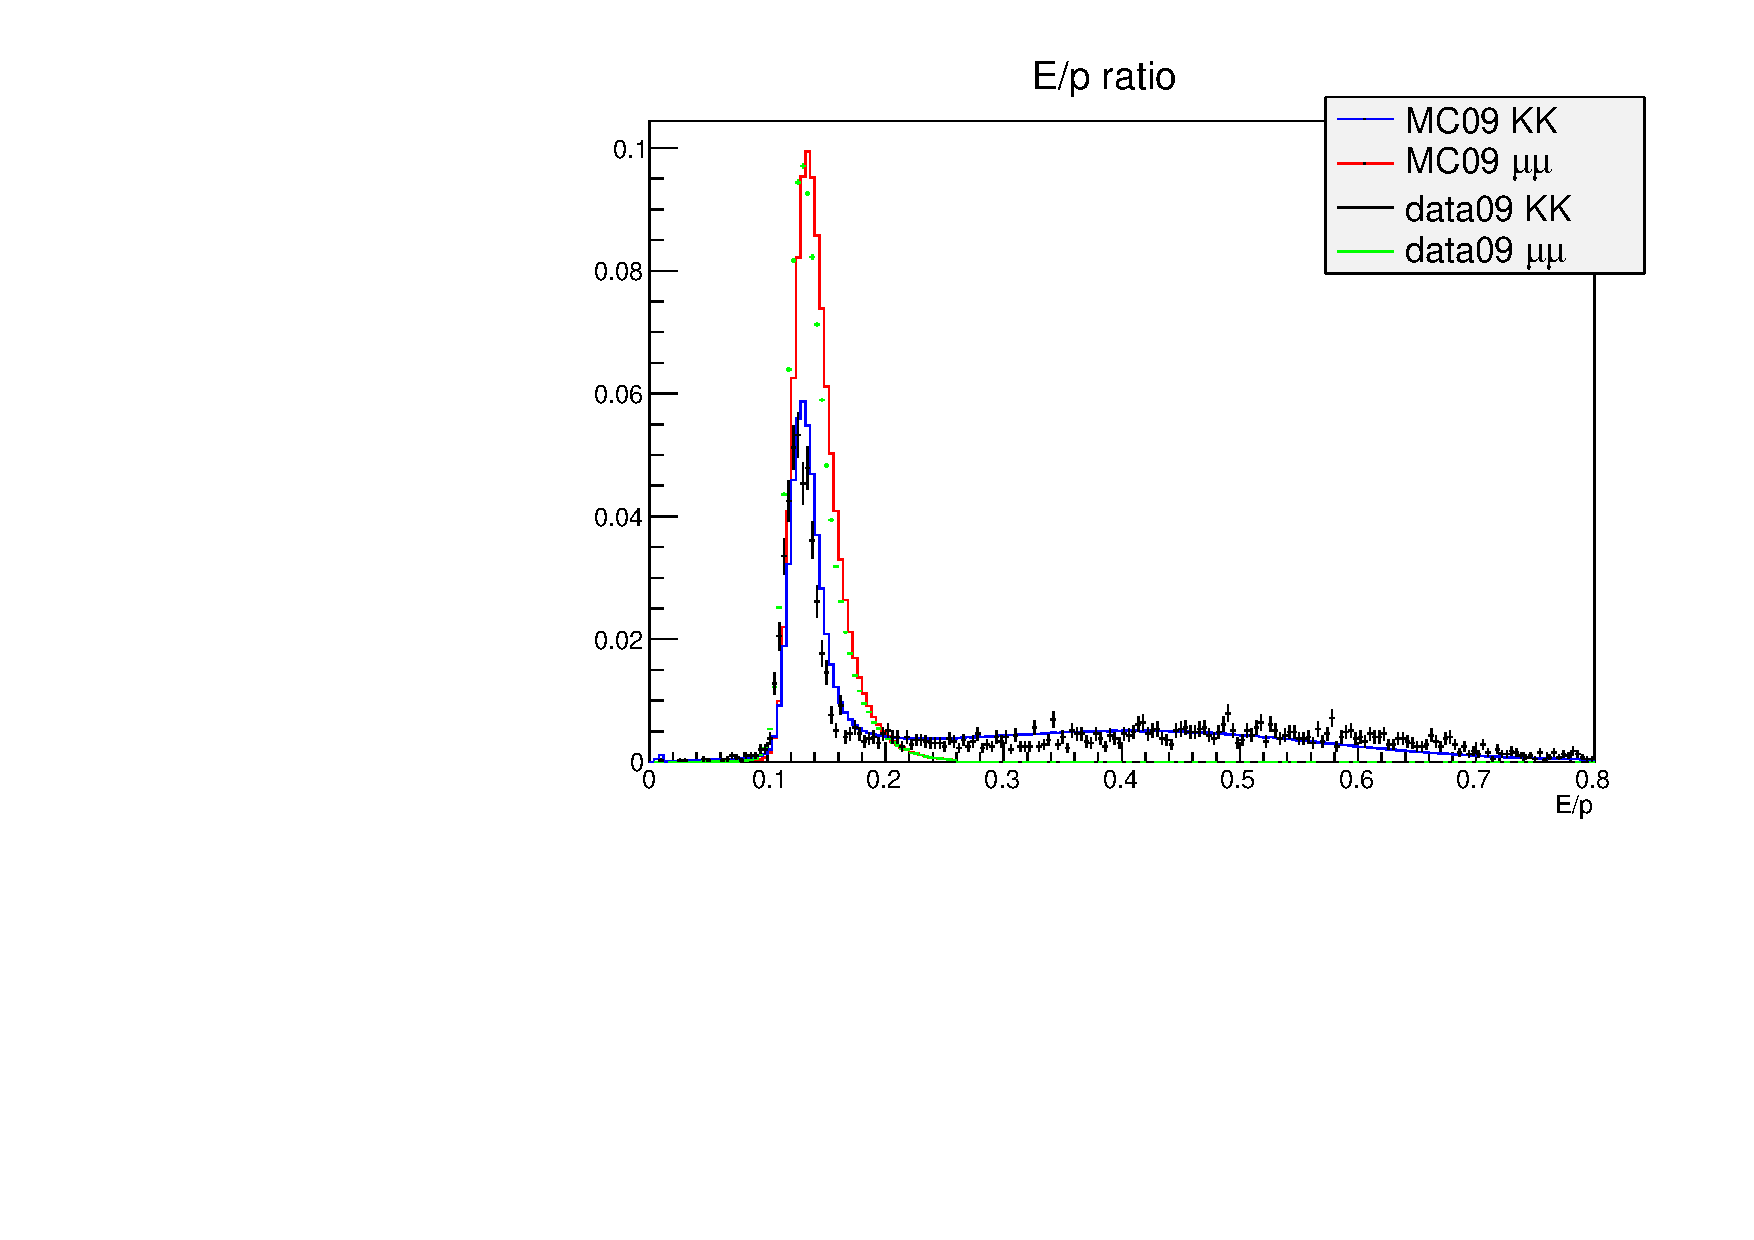
\includegraphics[width=0.48\textwidth]{fig/Ep.pdf}
  \caption{Muon or kaon momentum (left), E/p ratio (right)}
\end{center}
\end{figure}


For this selected tracks vertex fit is applied: all tracks must begin from single point.
Then kinematic fit was applied in two hypothesis for $\pi^+\pi^-\mu^+\mu^-$ ($\mu\mu$) and
$\pi^+\pi^-K^+K^-$ (KK) final state. 
\[
	P_{\psi(2S)} = P_{\pi^+} +  P_{\pi^-} + P_{K^+} +  P_{K^-}
\]

\[
	P_{\psi(2S)} = P_{\pi^+} +  P_{\pi^-} + P_{\mu^+} +  P_{\mu^-},
\]
here  $P_{\psi(2S)} = M_{\psi(2S)}\times (\sin(\alpha_{BEPC}/2),0,0, 1)$ ---
initialy four momentum of $\psi(2S)$;  here $M_{\psi(2S)} = 3.686108\
\mbox{GeV}$ is the PDG-2014 mass of the $\psi(2S)$ resonance,
$\alpha_{BEPC}=0.022$ is the beam crossing of BEPC-II. Choose KK or $\mu\mu$
hypothesis corresponding lower $\chi^2_{kin}$. Addition information for
particle identification used for TOF and MDC DeDx system.
$\chi^2_{PID} = \chi^2_{TOF} + \chi^2_{dE/dx}$. Additionally muons energy-momentum
ratio $E/p<0.26$ is demanded for $\mu\mu$ channel:
For $\mu\mu$ channel

\begin{minipage}{0.49\textwidth}
For kaon case:
\begin{itemize}
  \item $\chi^2_{kin}(KK) <200$
	\item $\chi^2_{kin}(KK) < \chi^2_{kin}(\mu\mu)$
	\item $\chi^2_{pid}(KK) < \chi^2_{pid}(\mu\mu)$
	\item $\chi^2_{pid}(KK) < \chi^2_{pid}(\pi\pi)$
\end{itemize}
\end{minipage}
\hfill
\begin{minipage}{0.49\textwidth}
For muon case:
\begin{itemize}
  \item $\chi^2_{kin}(\mu\mu) < 200$
	\item $\chi^2_{kin}(\mu\mu) < \chi^2_{kin}(KK)$
	\item $\chi^2_{pid}(\mu\mu) < \chi^2_{pid}(KK)$
	\item $\chi^2_{pid}(\mu\mu) < \chi^2_{pid}(\pi\pi)$
  \item $E/p<0.26$     
\end{itemize}
\end{minipage}

The final selection criteria are:
\begin{itemize}
\item $|M_{rec}(\pipi)-3097| < 90 MeV$
\item $\chi^2_{kin} < 40$
\item $\chi^2_{pid} < 20$
\end{itemize}

\section{Background analisis}

Inclusive Monte Carlo allow us to determine relevant background of $\psi(2S)$ decay (Table~\ref{tab:KKtopo}).
One can see the main background contribution come from  decay to $K_1(1270)$, $K^*(892)^0$, $K_{0,2}^*(1430)^0$ and
direct to $\pipi\KK$. 
Figure~\ref{fig:M012_Mrec} shows
 \begin{table}
   \centering
   \label{tab:KKtopo}
   \caption{Inclusive Monte Carlo 2009, $KK$-channel}
   \begin{tabular}{rrcl} \\
\#     &   count & final state & decay topology                      \\   \hline   
  1   &       1 & $\pi\pi \mu\mu$ & $  \psi(2S) \to \pipi (J/\psi \to \uu)                       $ \\ 
  2   &       2 & $\pi\pi KK$ & $  \psi(2S) \to (-K^*(892)^0 \to \pi^+ K-)(K_0^*(1430)^0 \to \pi^-K^+ +c.c.  $ \\ 
  3   &       2 & $\pi\pi KK$ & $  \psi(2S) \to (\rho(770)^0 \to \pipi )\KK                    $ \\ 
  4   &       2 & $\pi\pi KK$ & $  \psi(2S) \to \pi^+ (K_2^*(1430)^0 \to \pi^-K^+)K^-     +c.c.          $ \\ 
  5   &      14 & $\pi\pi KK$ & $  \psi(2S) \to (-K^*(892)^0 \to \pi^+ K^-)(K_2^*(1430)^0 \to \pi^-K^++c.c.  $ \\ 
  6   &      24 & $\pi\pi KK$ & $  \psi(2S) \to (K^*(892)^0 \to \pi^-K^+)(-K^*(892)^0 \to \pi^+ K^-)+c.c.   $ \\ 
  7   &      25 & $\pi\pi KK$ & $  \psi(2S) \to \pipi \KK                                $ \\ 
  8   &      27 & $\pi\pi KK$ & $  \psi(2S) \to K^-(K_1(1270)^+ \to (\rho(770)^0 \to \pipi )K^+)+c.c.    $ \\ 
  9   &      53 & $\pi\pi KK$ & $  \psi(2S) \to K^+(K_1(1270)^- \to \pipi K^-)      +c.c.          $ \\ 
 10   &      73 & $\pi\pi KK$ & $  \psi(2S) \to \pi^-(-K^*(892)^0 \to \pi^+ K^-)K^+   +c.c.             $ \\ 
 11   &     112 & $\pi\pi KK$ & $  \psi(2S) \to K^-(K_1(1270)^+ \to \pi^+ (K^*(892)^0 \to \pi^-K^+))   +c.c. $ \\ 
 12   &     248 & $\pi\pi KK$ & $  \psi(2S) \to K^+(K_1(1270)^- \to \pi^-(-K_0^*(1430)^0 \to \pi^+ K^-)) +c.c.$ \\ 
 13   &    2801 & $\pi\pi KK$ & $  \psi(2S) \to \pipi (J/\psi \to \KK )                       $ \\ \hline
 \end{tabular}
 \end{table}

 \begin{table}
   \centering
   \label{tab:KKtopo}
   \caption{Inclusive Monte Carlo 2009, $\mu\mu$-channel}
   \begin{tabular}{rrrl} \\
  \#   &  count & final state & decay topology                      \\   \hline   
  1&        1 &$ \gamma\pi\pi\pi\pi        $ &$ \psi(2S) \to \pipi(J/\psi \to \gamma(f_2(1270) \to \pipi))       $\\ 
  2&        1 &$ ee\mu\mu\gamma\gamma\gamma$ &$ \psi(2S) \to (\pi_0 \to \ee\gamma)(\pi_0 \to \gamma\gamma)(J/\psi \to \uu)    $\\ 
  3&        1 &$ \mu\mu\mu\mu\gamma        $ &$ \psi(2S) \to (\eta \to \uu\gamma)(J/\psi \to \uu)              $\\ 
  4&        1 &$ \pi\pi\pi\pi              $ &$ \psi(2S) \to \pipi\pipi                           $\\ 
  5&        1 &$ ee\mu\mu\gamma            $ &$ \psi(2S) \to (\eta \to \ee\gamma)(J/\psi \to \uu)              $\\ 
  6&        1 &$ \gamma\pi\pi\pi\pi        $ &$ \psi(2S) \to \pipi(J/\psi \to \gamma(f_2(2150) \to \pipi))       $\\ 
  7&        2 &$ \pi\pi\pi\pi              $ &$ \psi(2S) \to \pi^+(b_1(1235)^- \to \pi^-(\omega(782) \to \pipi)) +c.c.   $\\ 
  8&        2 &$ \mu\mu                    $ &$ \psi(2S) \to \uu                                 $\\ 
  9&        3 &$ \pi\pi\pi\pi              $ &$ \psi(2S) \to \pi^-(a_2(1320)^+ \to (\rho(770)^0 \to \pipi)\pi^+) +c.c.  $\\ 
 10&        5 &$ \gamma\pi\pi\pi\pi        $ &$ \psi(2S) \to \pipi(J/\psi \to \gamma(f_4(2050) \to \pipi))       $\\ 
 11&       13 &$ \pi\pi\pi\pi              $ &$ \psi(2S) \to (\rho(770)^0 \to \pipi)\pipi                 $\\ 
 12&       77 &$ \mu\mu\gamma \pi\pi       $ &$ \psi(2S) \to (\eta \to \gamma\pipi)(J/\psi \to \uu)              $\\ 
 13&      589 &$ \pi\pi\pi\pi              $ &$ \psi(2S) \to \pipi(J/\psi \to \pipi)                     $\\ 
 14&   675597 &$ \mu\mu\pi\pi              $ &$ \psi(2S) \to \pipi(J/\psi \to \uu)                     $\\ \hline
 \end{tabular}
 \end{table}

\begin{figure}
	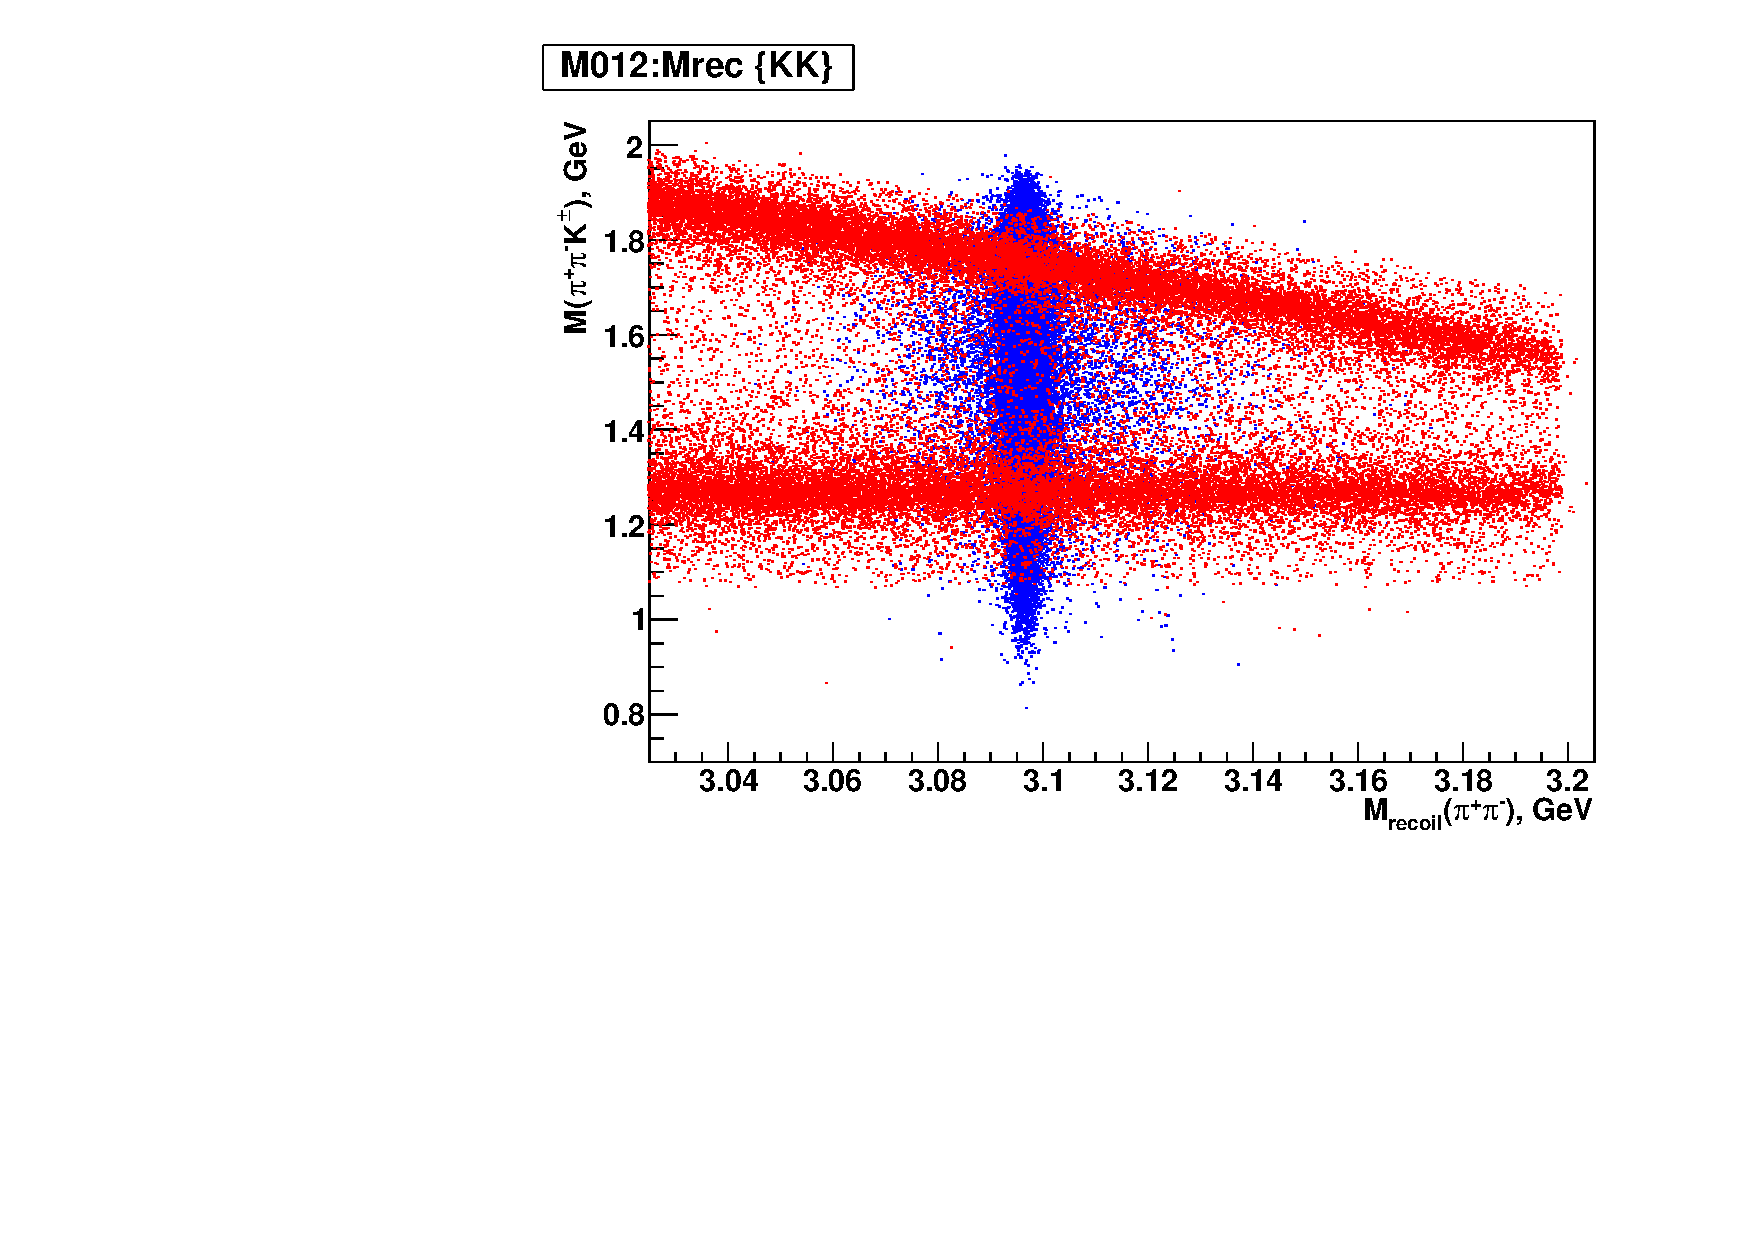
\includegraphics[width=\textwidth]{fig/M012_Mrec-color.pdf}
	\caption{Axis X -recoil invariant mass of $\pi^+\pi^-$,  axis y - invariant
	mass of $\pi^+\pi^-K^\pm$.  Blue is for $\psi^\prime \to J/\psi \pi^+\pi^-
	\to K^+K^-\pi^+\pi^-$. Red for $\psi^\prime \to K_1(1270)^\mp K^\pm  \to
	K^+K^-\pi^+\pi^-$}
  \label{fig:M012_Mrec}
\end{figure}

%\begin{table}
%	\begin{tabular}{lc} \hline
%		process &  probability \\ 
%		$\psi(2S) \to K_1^{\pm}(1270) K^{\mp}$  & $0.0005 \times 2$ \\ 
%		$\psi(2S) \to K^+K^-\pi^+\pi^-$   & $7.5 \times 10^{-4}$  \\
%		$\psi(2S) \to \rho^0 K^+K^-$   & $2.2 \times 10^{-4}$  \\
%	$\psi(2S) \to  K^\pm \pi^\mp K^{*}(892)^0$  &  $6.7\pm10^{-4}$
%	\end{tabular}
%\end{table}



The result of selection is shown at Figure~\ref{fig:mc09-Mrec} for inclusive
Monte Carlo; Figure~\ref{fig:data-Mrec} for the data and in
Talbe~\ref{tab:res09}.  The ratio of registration efficiency
$\varepsilon_{KK}/\varepsilon_{\mu\mu}= 1.063 \pm 0.002$ is measured by MC
simulation fo $10^7$ decays.  There is a good agreement with setup value of
$B(KK)/B(\mu\mu)$ ratio and measured result for Monte Carlo, but there is 13\%
($2\sigma$ deviation) difference between measured and PDG value.

\begin{table}
  \centering
  \label{tab:res09}
  \caption{Selection result}
  \begin{tabular}{lll} 
                          & Monte Carlo 2009 & data 2009      \\  \hline
  $ N_{tot}^{KK}$         & 3384             &    3747        \\            
  $ N_{fit}^{KK}$         & $2840\pm65$      &    $3586\pm60$ \\
  $ N_{bg}^{KK}$          & $544\pm23$       &          $161 \pm 13$   \\
  $ N_{tot}^{\mu\mu}$     & $676294$         &       659534   \\
  $ N_{fit}^{\mu\mu}$     & $676294\pm822$   &       $659534 \pm 812$   \\
  $ N_{bg}^{\mu\mu}$      & $0           $   &       0    \\
  $ N_{fit}^{KK}/N_{fit}^{\mu\mu}$& $(4.20 \pm 0.09)\times10^{-3} $ & $(5.44 \pm 0.09)\times 10^{-3}$  \\
  $\varepsilon_{KK}/\varepsilon_{\mu\mu}$ & $1.063 \pm 0.002$ &  $1.063 \pm 0.002$  \\
    $ B_{KK}/B_{\mu\mu}(meas)$   & $(3.95 \pm 0.09)\times 10^{-3}$  & $(5.12 \pm 0.09)\times 10^{-3}$ \\
    $ B_{KK}/B_{\mu\mu}(set)$   & $4.00\times 10^{-3}$  & $(4.53 \pm 0.29)\times 10^{-3}$
\end{tabular}
\end{table}

\begin{figure}
\begin{center}
  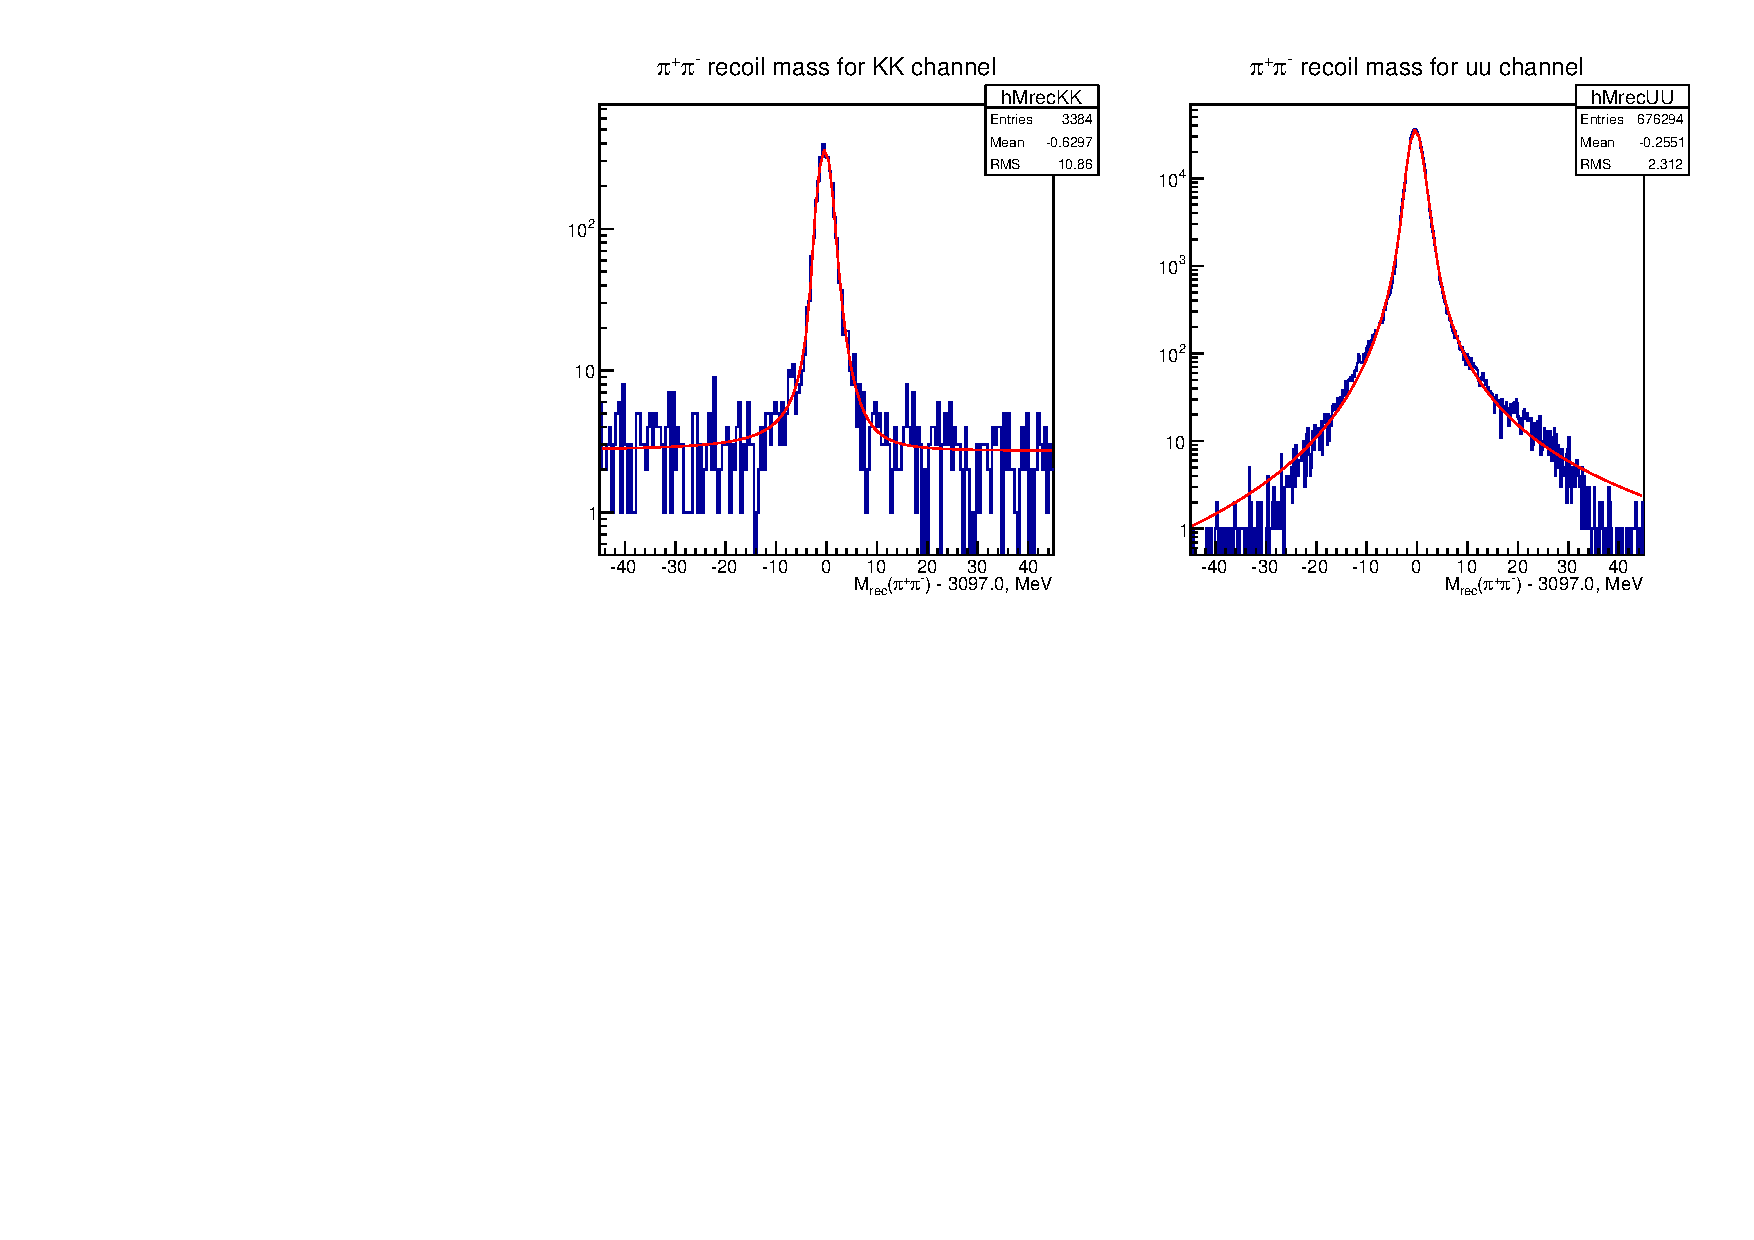
\includegraphics[width=\textwidth]{fig/mc09-Mrec90MeV.pdf}
  \caption{Inclusive MC2009. Pion recoil mass for $\KK$ channel (left) and $\uu$ channel (right)}
  \label{fig:mc09-Mrec}
\end{center}
\end{figure}
\begin{figure}
\begin{center}
  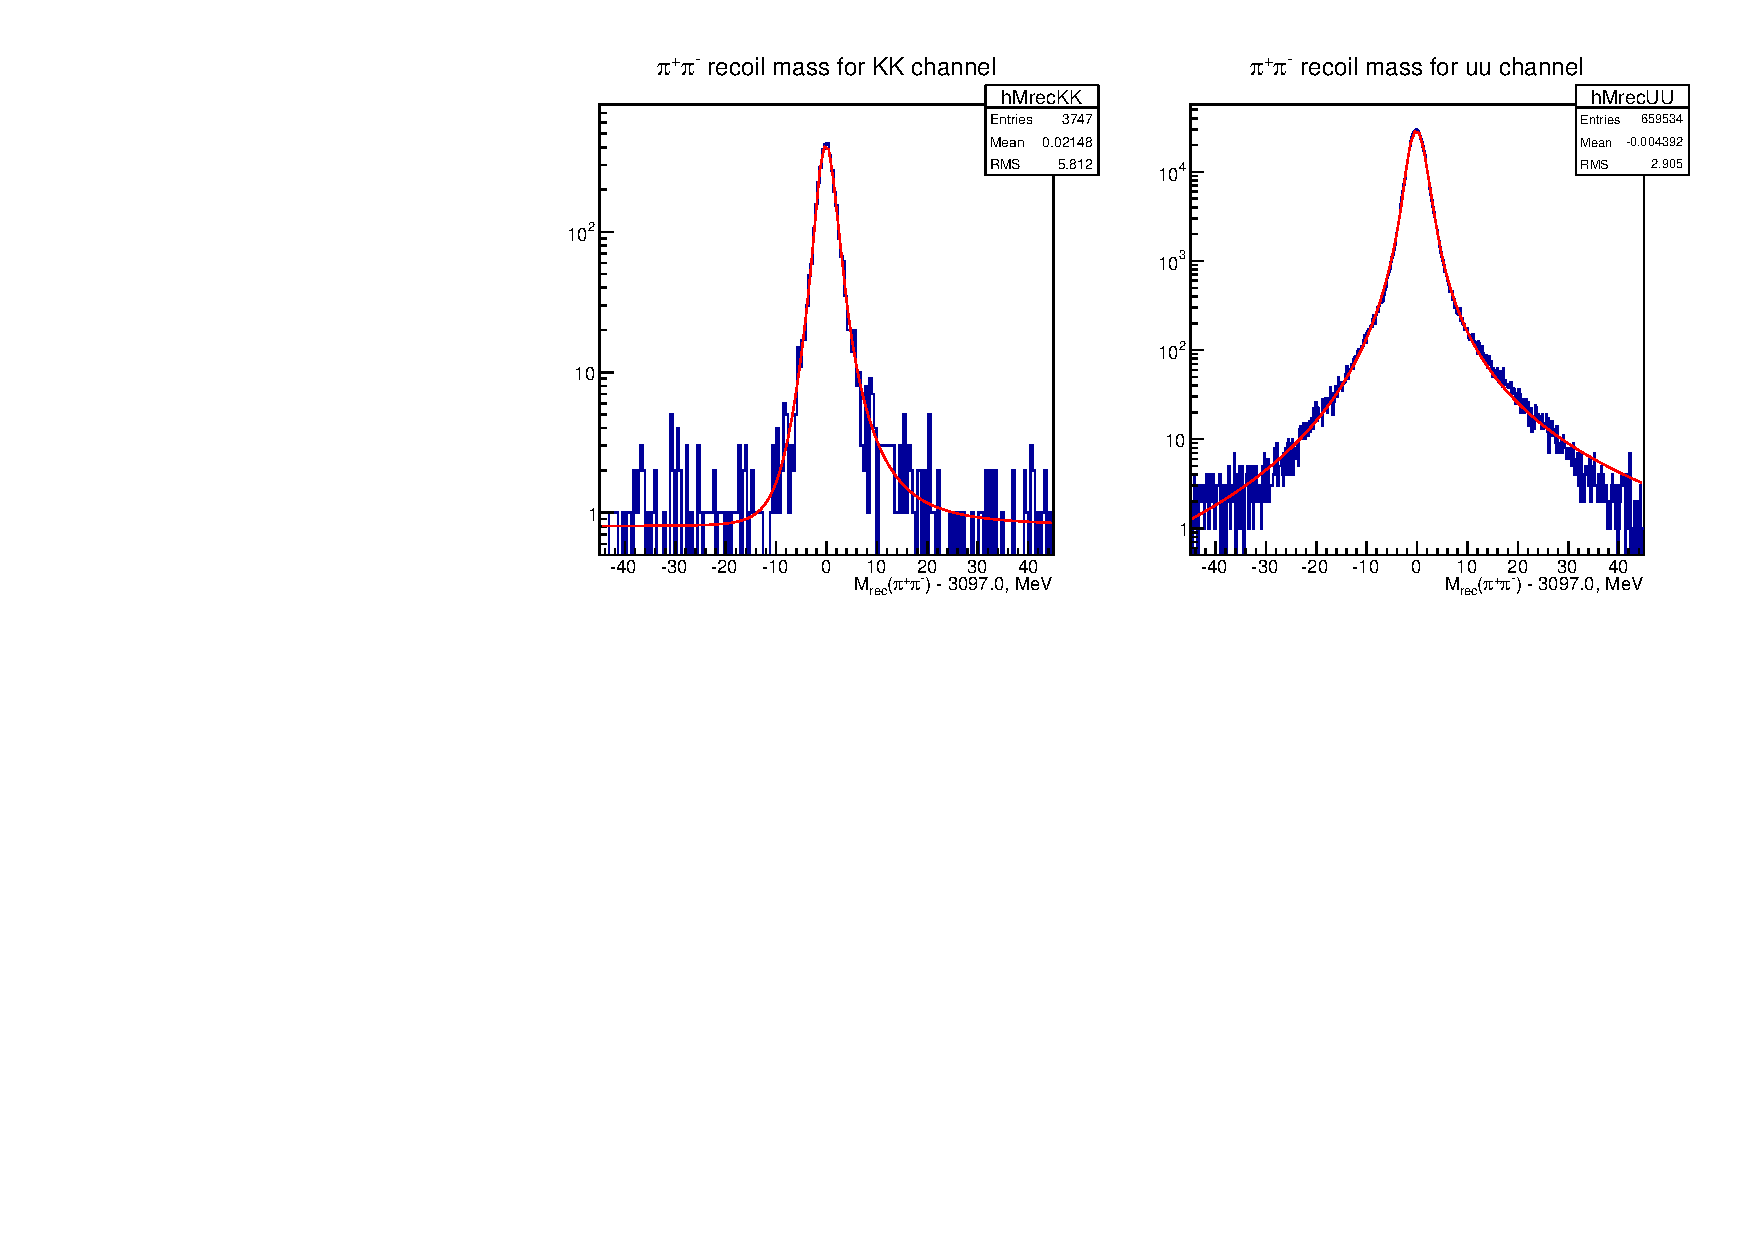
\includegraphics[width=\textwidth]{fig/data09-Mrec90MeV.pdf}
  \caption{Data 2009. Pion recoil mass for $\KK$ channel (left) and $\uu$ channel (right)}
  \label{fig:data09-Mrec}
\end{center}
\end{figure}
\begin{figure}
\begin{center}
  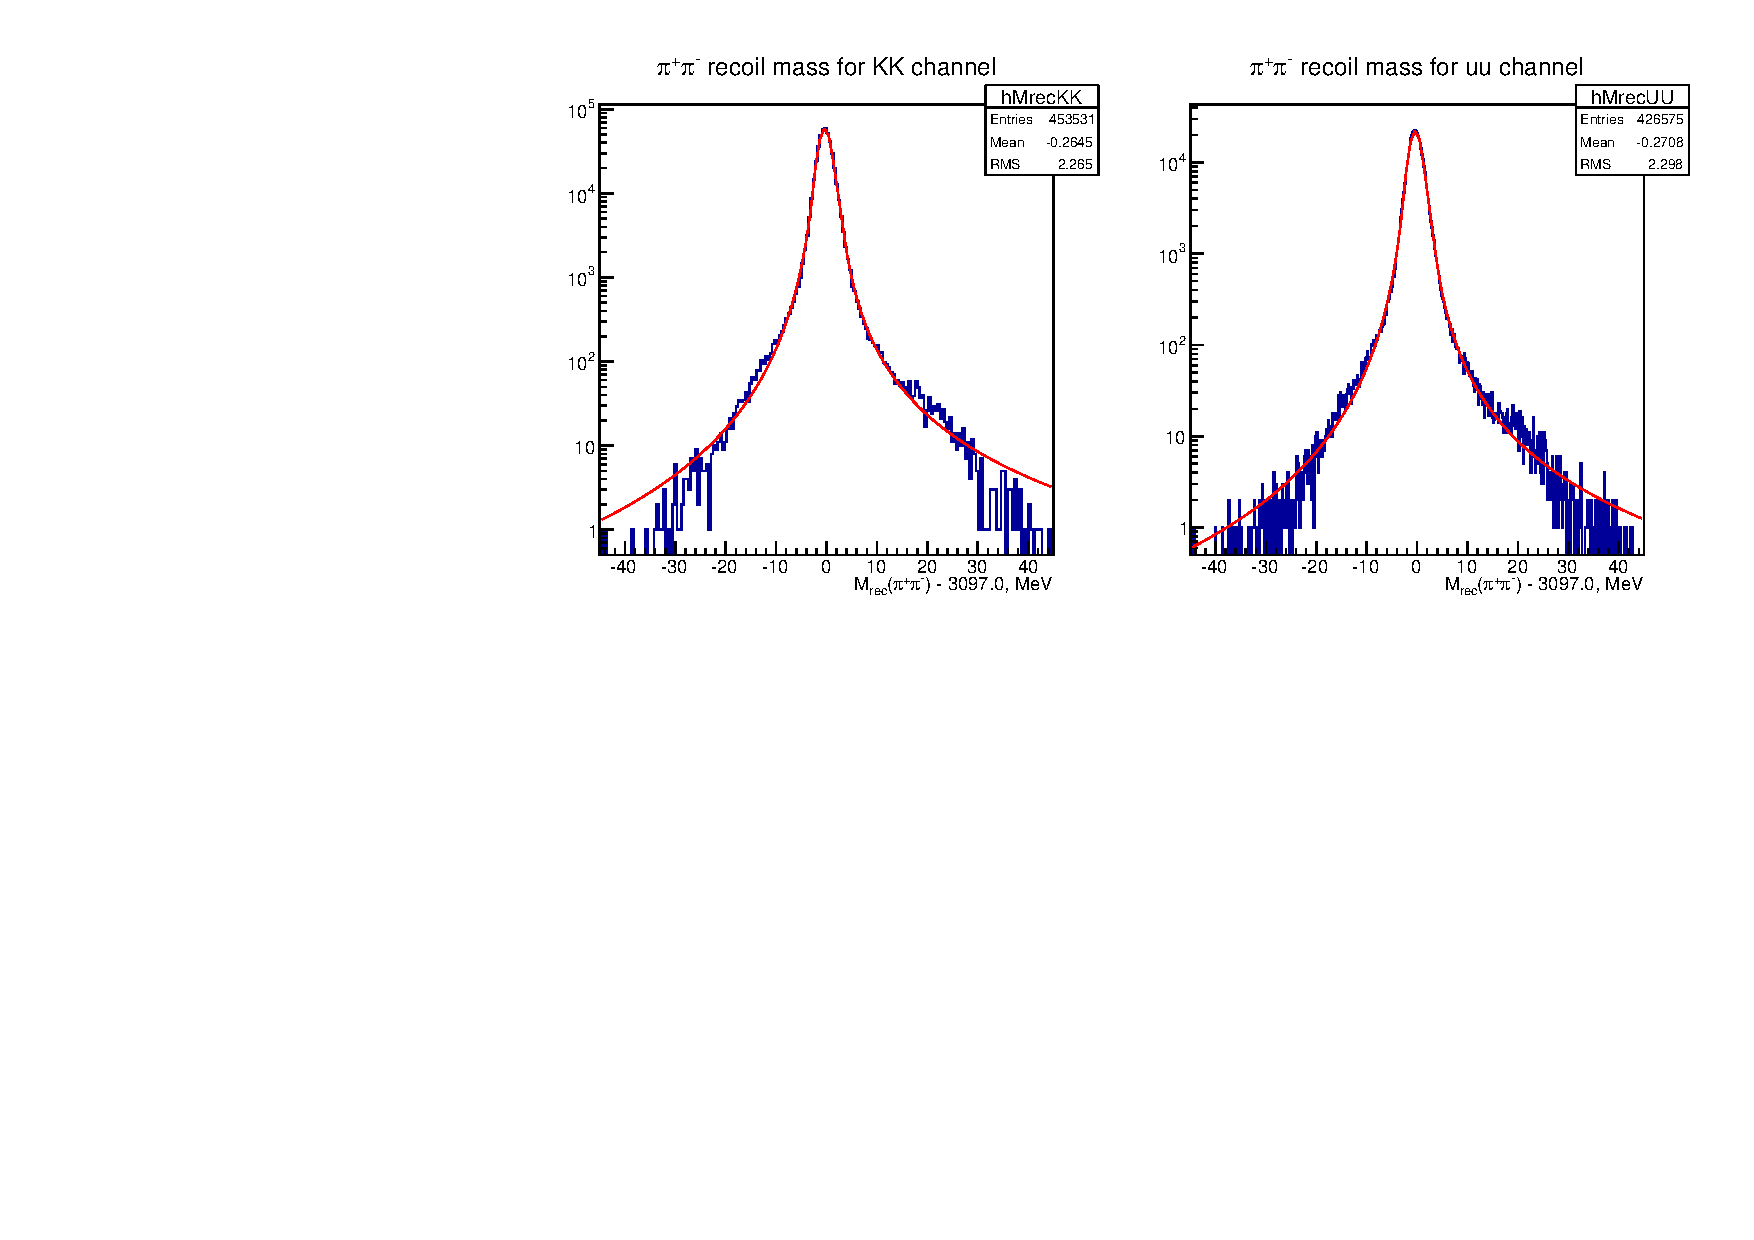
\includegraphics[width=\textwidth]{fig/mcKKuu-Mrec90MeV.pdf}
  \caption{Exclusive MC2009. Pion recoil mass for $\KK$ channel (left) and $\uu$ channel (right)}
  \label{fig:mcexcl09-Mrec}
\end{center}
\end{figure}

\begin{figure}
\begin{center}
  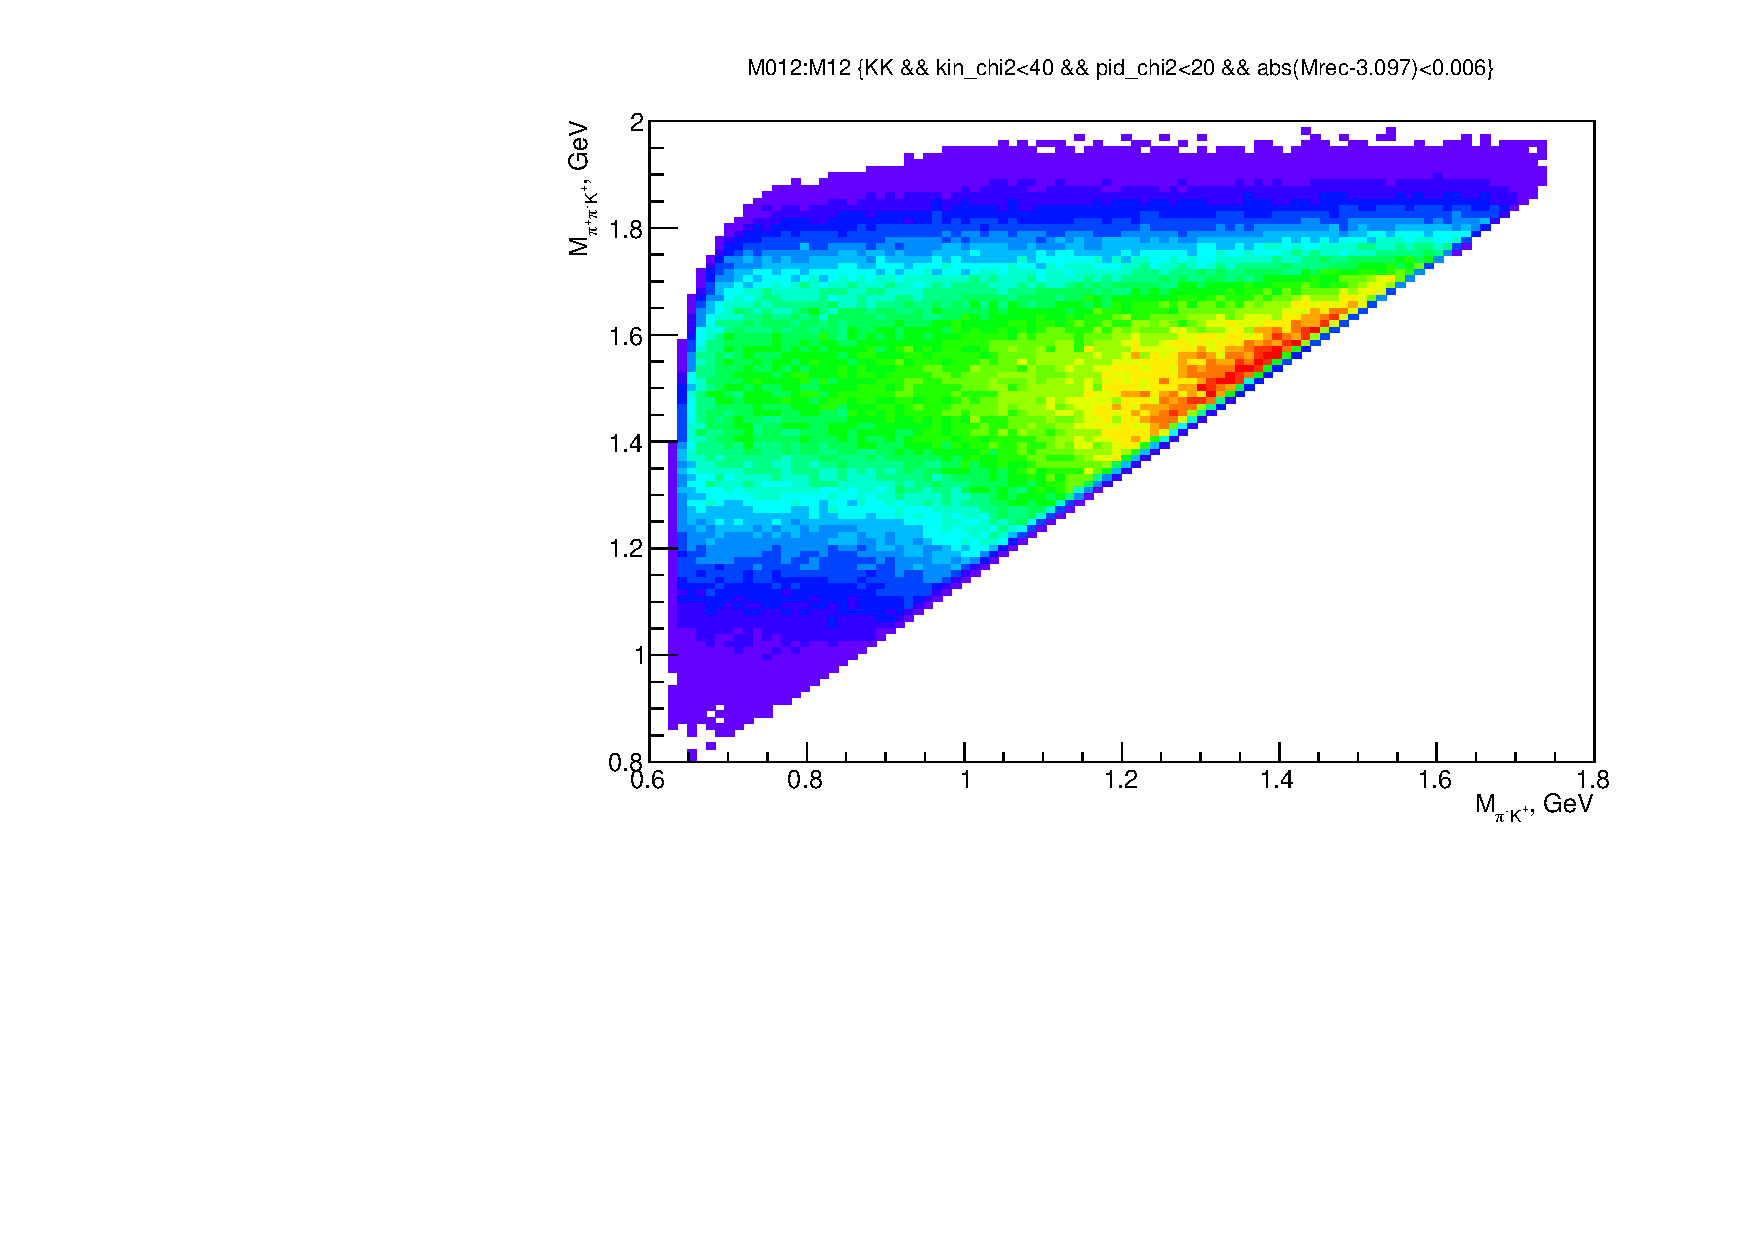
\includegraphics[width=0.49\textwidth]{fig/dalitz-KK2.pdf}
  \hfill
  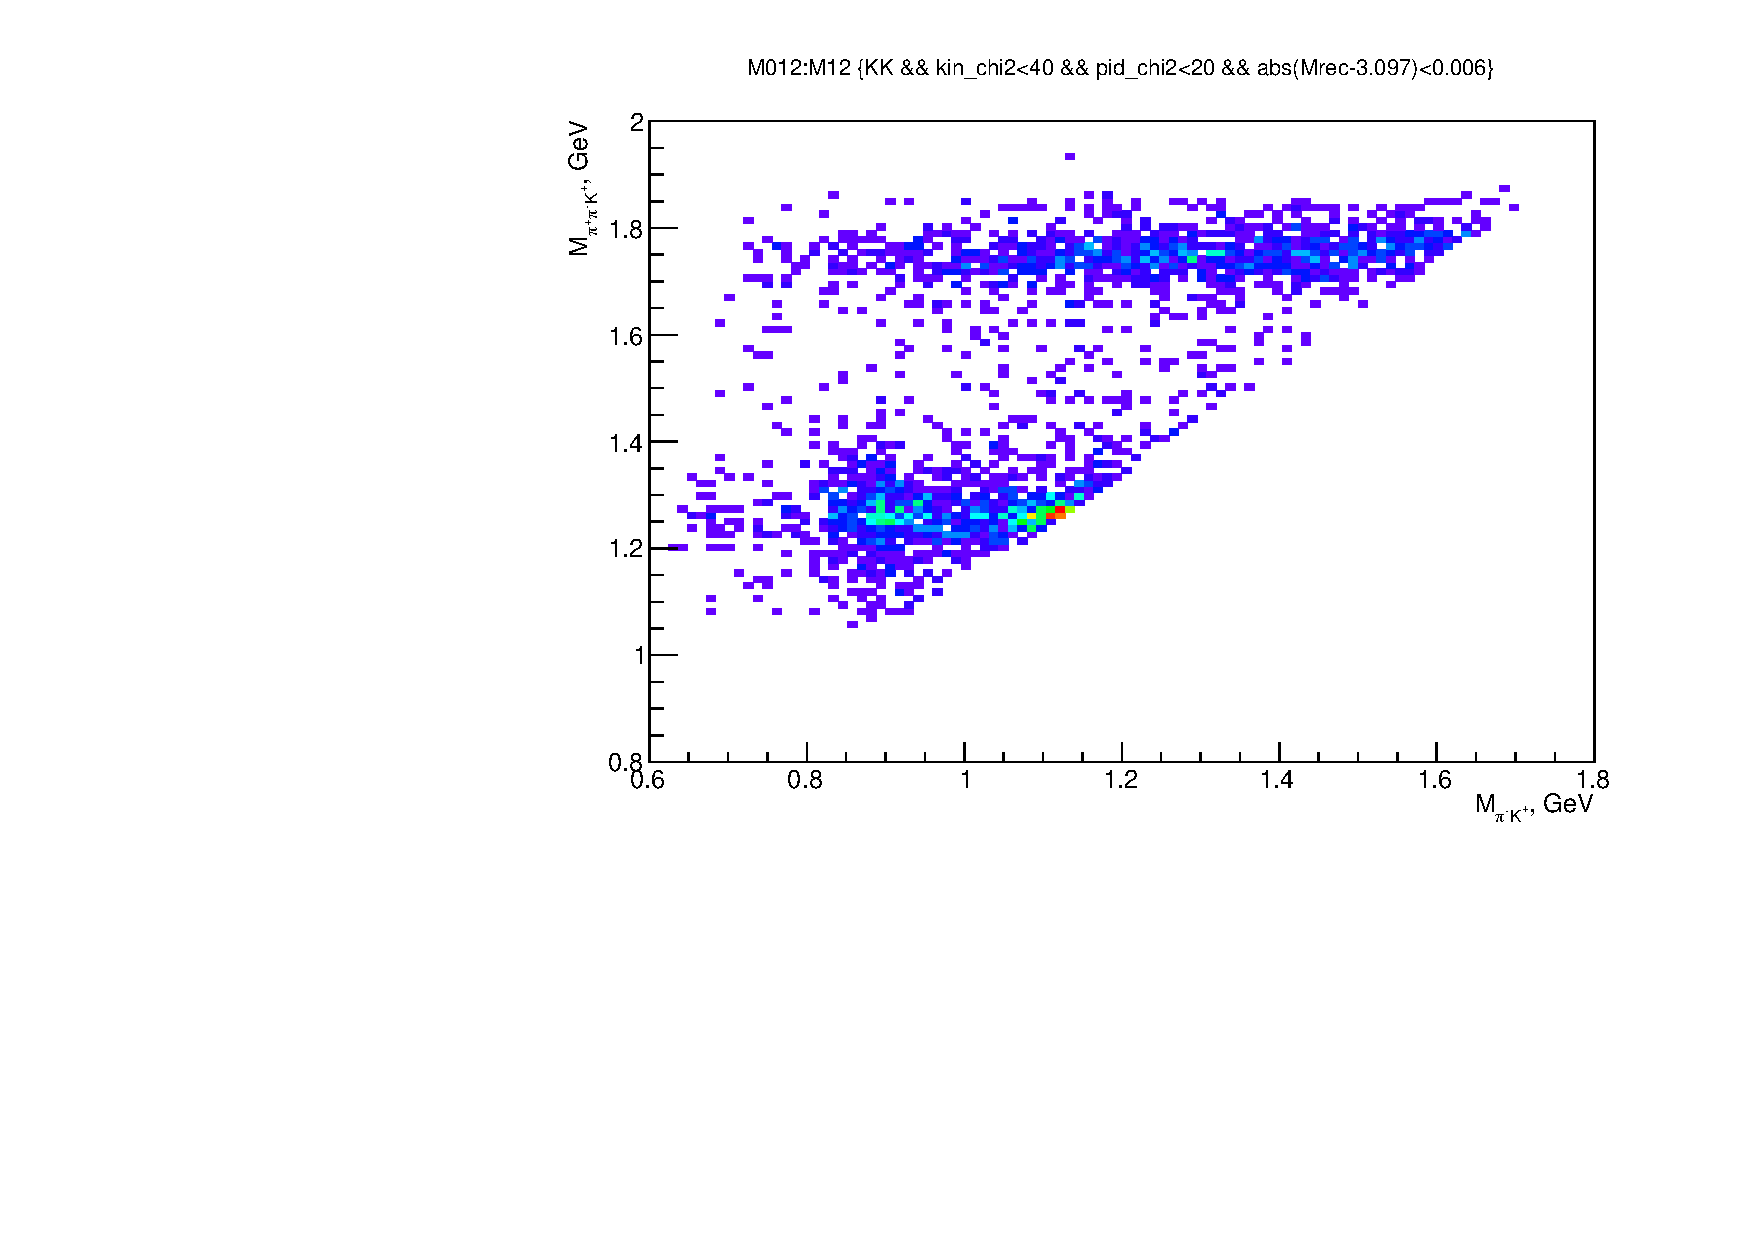
\includegraphics[width=0.49\textwidth]{fig/dalitz-bg2.pdf}
  \caption{}
\end{center}
\end{figure}

\section{Interference with the background}
Оценим максимальную величину интерференции между сигналом и фоном.

\begin{eqnarray}
  dN_{sig} & = & \epsilon L \sigma_{\psi(2S)} |A(x, y) BW(W)|^2  dW dx dy \\
  dN_{bg} & = & \epsilon L \sigma_{\psi(2S)}  |B(x, y)|^2  dW dx dy,
\end{eqnarray}

here BW(x) is Breight-Wigner function:
\begin{equation}
  BW(W) =  \frac{M \Gamma}{M^2-W^2 - iM\Gamma};
\end{equation}
\begin{eqnarray}
W & = & M_{rec} = \sqrt{(P_{\pi^+}+ P_{\pi^-})^2}, \nonumber \\
x & = & M_{\pipi K^+} = \sqrt{(P_{\pi^+}+ P_{\pi^-} + P_{K^+})^2}, \nonumber \\ 
y & = & M_{\pi^- K^+} = \sqrt{(P_{\pi^-} + P_{K^+})^2}, \nonumber \\
\end{eqnarray}


The interference contribution proportional:
\begin{equation}
  2 |A(x,y) B(x,y) BW(M_{rec})| \cos\phi,
\end{equation}
where $\phi$ is an appropriate phase difference between two amplitudes.


And number of events:
\begin{equation}
  dN_{int} = \epsilon L \sigma_{\psi(2S)} 2\cos(\phi)|A(x,y) B (x,y)|\frac{M \Gamma}{\sqrt{(M^2-W^2)^2 + M^2\Gamma^2}} dW dx dy
\end{equation}


\begin{equation}
  \int_{0}^{\infty}\frac{M^2 \Gamma^2}{(M^2-W^2)^2 + M^2\Gamma^2} dW = \frac{\pi}{2} \Gamma
\end{equation}

\begin{equation}
  \int_{0}^{\infty}\frac{M \Gamma}{\sqrt{(M^2-W^2)^2 + M^2\Gamma^2}} dW \approx \Gamma \ln\frac{M}{\Gamma}
\end{equation}

\begin{equation}
  N_{int} = \epsilon L \sigma_{\psi(2S)} 2\cos(\phi) \Gamma \ln\frac{M}{\Gamma}\int |A(x,y) B (x,y)|dxdy
\end{equation}
\begin{equation}
  N_{sig} = \epsilon L \sigma_{\psi(2S)} \frac{\pi}{2} \Gamma \int |A(x,y)|^2 dxdy
\end{equation}
\begin{equation}
  N_{bg} = \epsilon L \sigma_{\psi(2S)} \Delta W \int |B(x,y)|^2 dxdy
\end{equation}

\begin{equation}
  \frac{N_{int}}{N_{sig}} = 2\cos\phi\ln\frac{M}{\Gamma} 
  \sqrt{\frac{N_{bg}}{N_{sig}}\frac{2 \Gamma}{\pi \Delta W}} 
  \frac{\int |A(x,y) B (x,y)|dxdy}{\int |A(x,y)|^2 dxdy\int |B(x,y)|^2 dxdy}
\end{equation}

Using Monte Carlo for background $\psi(2S) \to K_1(1270) X \to \pipi KK $ and for the signal $\psi(2S) \to J/\psi\pipi \to \pipi KK $ one can receive:
\begin{equation}
  \frac{\int |A(x,y) B (x,y)|dxdy}{\int |A(x,y)|^2 dxdy\int |B(x,y)|^2 dxdy} \approx 0.5
\end{equation}

Then fraction of interference
\begin{equation}
  \frac{N_{int}}{N_{sig}} \le 2 \cdot 0.5 \ln\frac{M}{\Gamma} 
    \sqrt{\frac{N_{bg}}{N_{sig}}\frac{2 \Gamma}{\pi \Delta W}}   \approx 0.06
\end{equation}
here $\Gamma = \Gamma_{J/\psi} = 0.093$~MeV, $M= M_{J/\psi}=3097$~MeV, $N_{bg}=160$, $N_{sig} = 3586$, $\Delta W = 90$~MeV 




\subsection{Fit for recoil mass}

In order to fit $\pi^+\pi^-$ recoil mass modified Crystal Ball \cite{CrystalBallFunc}functin with right and left tail is used:
\begin{equation}
	%mCristalBall(x, N, \alpha_{el},\alpha_{l}, n_l,  \alpha_{er}, \alpha_r,  n_r )  = 	N \left\{
	f_{CB}(x)  = 	\left\{
		\begin{array}{lrrr}
			A_l(B_l - x)^{-n_l},  & -\infty &   x <&   -\alpha_l \\
			A_{el}\exp(\alpha_{el}x), &  -\alpha_l & < x  < &-\alpha_{el} \\
			\exp( - x^2/2),  &  - \alpha_{el} & < x < & \alpha_{er} \\
			A_{er}\exp(-\alpha_{er}x), &  \alpha_{el} & < x < & -\alpha_{r} \\
			A_r(B_r + x)^{-n_r}, &   \alpha_r & < x < & \infty \\
		\end{array}
		\right., 
\end{equation}
\begin{equation}
	\begin{array}{lcl}
		A_{er, el} & = &  \exp(\alpha_{er, el}^2/2) \\
		B_{ r, l}  &  = & n_{r, l}/ \alpha_{er, el} - \alpha_{r, l}
	\end{array}
\end{equation}


Fit function is
\begin{equation}
N f_{CB}\left( \frac{m - M}{\sigma},  \alpha_{el},\alpha_{l}, n_l,  \alpha_{er}, \alpha_r,  n_r\right)  +  N_{bg}
\end{equation}








\begin{figure}
	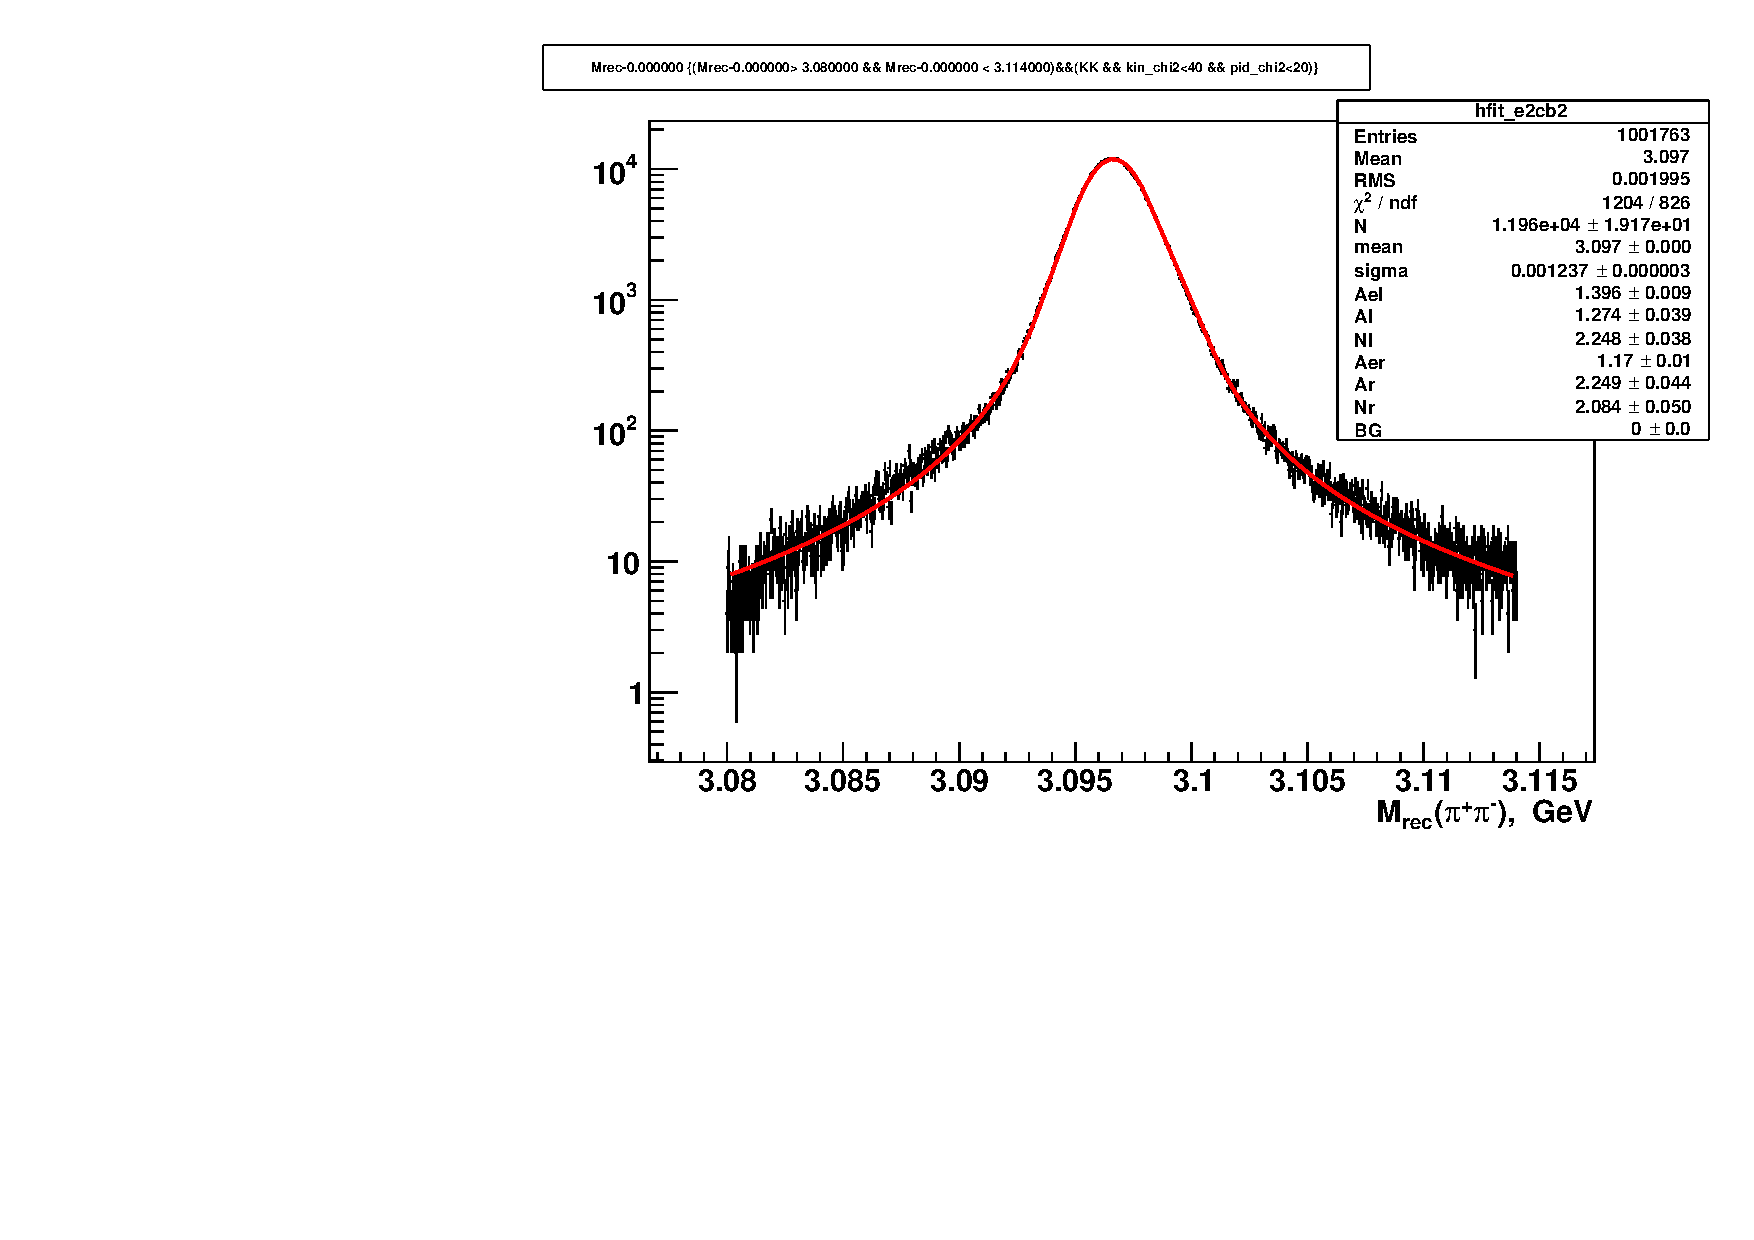
\includegraphics[width=\textwidth]{fig/Mrec_fit_double_exp_double_crystal_ball.pdf}
	\caption{Recoil invariant mass of $\pi^+\pi^-$ fitted by 
		modified Crystall Ball function}
\end{figure}

\end{document}

